
%5%%5%%5%%5%%5%%5%%5%%5%%5%%5%%5%%5%%5%%5%%5%%5%%5%%5%%5
%                     Estratégia                       %
%5%%5%%5%%5%%5%%5%%5%%5%%5%%5%%5%%5%%5%%5%%5%%5%%5%%5%%5

\chapter{Estratégia para identificação automática das soft skills}

\label{chap:metrics}

Conhecemos a importância das soft skills para o processo de contratação na subseção \ref{subsec:ss-importance}. Nesse contexto, é comum que as empresas encontrem dificuldades para identificar habilidades de seus candidatos. Isso porque identificar soft skills é uma tarefa que consome tempo, pois é necessário conhecer o indivíduo e seu comportamento durante um determinado período, até ter condições de reconhecer suas habilidades. Para minimizar esse problema, apresentamos uma estratégia que foca no papel do programador de software e visa identificar soft skills de maneira automática.

%Dividimos a estratégia para identificaçao automática de soft skills em três passos: (1) Levantamento de soft skills, (2) Conceituação das soft skills, (3) Desenvolvimento de métricas para identificação das soft skills. Podemos observar esses passos na Figura \ref{fig:estrategia}.

%\begin{figure}[h*]
%\centering
%\caption{\small Estratégia para identificaçao automática de soft skills} 
%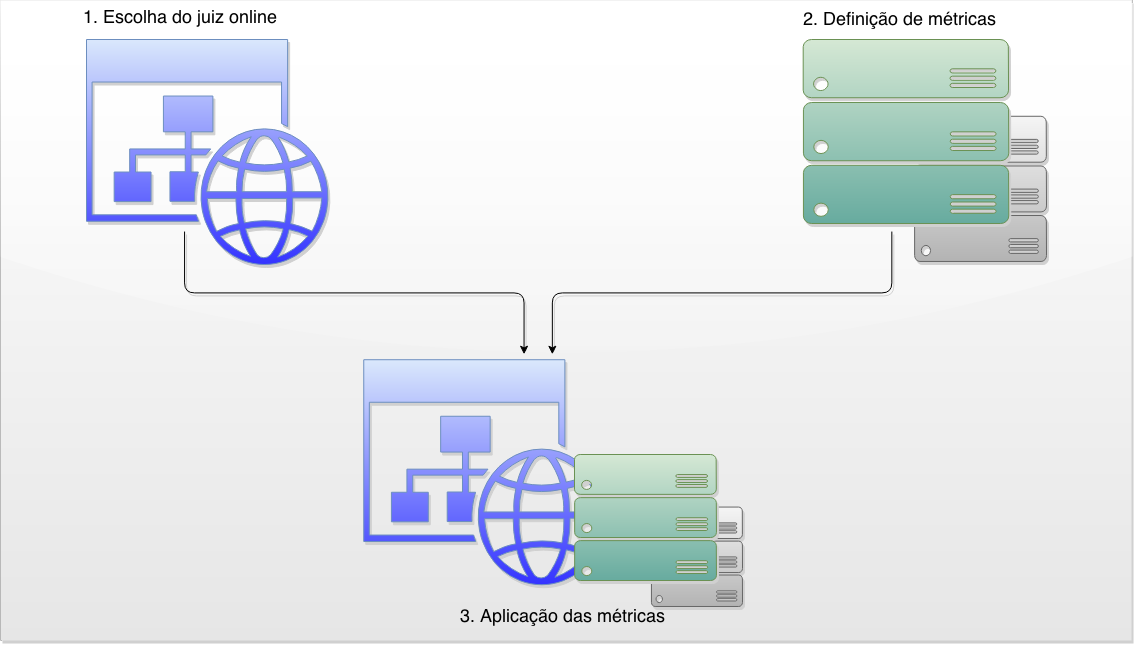
\includegraphics[width=.9\textwidth]{estrategia.png}
%\label{fig:estrategia}
%\end{figure}

Essa estratégia está baseada, inicialmente, em entender o significado das soft skills, para então buscar formas de identificá-las.
Até este ponto, fizemos o levantamento de algumas soft skills do referido papel, tema abordado no capítulo \ref{chap:research}. Em seguida, no capítulo \ref{chap:concepts}, formamos uma base teórica e conceitual a respeito das soft skills.
Agora iremos detalhar a estratégia em si.

Para atingir o objetivo de identificar soft skills de maneira automática, levamos em consideração alguns pontos. Primeiramente, sabemos que é preciso conhecer o comportamento do indivíduo para reconhecer suas habilidades. Portanto, propomos que, para identificar as soft skills de um programador, é necessário observá-lo em suas atividades de programação. Além disso, como a identificação deve ocorrer automaticamente, precisamos utilizar um ambiente que possibilite a coleta automática de informações a respeito do comportamento de um programador.

Assim, nossa estratégia consiste no desenvolvimento de métricas que atribuem uma pontuação para cada soft skill de um programador. O ambiente em que podemos coletar essas métricas automaticamente é um juiz online, sistema no qual os usuários praticam atividades de programação. Esse tipo de sistema possui uma base de dados que guarda as interações de seus usuários, as quais podem ser analisadas a partir das referidas métricas, representando uma alternativa para identificação das soft skills.

%Then, we propose to use the past interaction of the student to identify soft skills by analyzing their previous interaction history based on their concepts and making use of metrics that can represent an alternative to know a person. As a source for this metrics, one might rely on online programming tools, since these systems allow the evaluation of its user's behavior. A popular category of this kind of system is the online judges. In subsection 3.1, we present the online judge system that we use in this paper.

%Portanto, dividimos a estratégia para identificaçao automática de soft skills em três passos: (1) Escolha de um juiz online, (2) Desenvolvimento de métricas, (3) Coleta de métricas utilizando a base de dados do juiz online. Podemos observar esses passos na Figura \ref{img:strategy}.

A Figura \ref{fig:estrategia} ilustra nossa estratégia, explicando-a em três passos.
Na seção \ref{sec:huxley}, tratamos das principais características de um juiz online e apresentamos o sistema que adotamos nesta dissertação, abordando o passo 1. Adicionalmente, na seção \ref{sec:metrics}, propomos as métricas para identificação de soft skills nos usuários de um juiz online, constituindo o passo 2. Já no passo 3, explicamos a aplicação das métricas e como obter as pontuações de cada soft skill dos usuários do juiz online, através do exemplo da seção \ref{sec:exemplo-metricas}.

\section{Juiz online} 
\label{sec:huxley}

Juiz online é um sistema que disponibiliza um conjunto de problemas de programação a serem resolvidos através da criação e codificação de algoritmos. O usuário do sistema pode acessar os problemas e submeter soluções para os mesmos. O juiz online avalia essas submissões testando-as de acordo com um conjunto de casos de teste predefinidos. Se a submissão passa por todos os casos de teste, o sistema a avalia como correta. Caso contrário, o sistema avalia a submissão de acordo com um tipo de erro, por exemplo, resposta errada, erro de compilação, tempo limite excedido, etc.

Nesse contexto, ao interagir com o sistema, os programadores geram dados que podemos coletar e aplicar a métricas, visando identificar soft skills automaticamente.
São exemplos de juízes online os sites de competições e suporte à correção de código, tais como CodeAcademy (\textit{codeacademy.com}), CodeChef (\textit{codechef.com}), Code Avengers (\textit{codeavengers.com}), etc.
Outros sistemas similares são os repositórios de cursos Khan Academy (\textit{khanacademy.org}), Udacity (\textit{udacity.com}) e CodeSchool (\textit{codeschool.com}).
Neste estudo, adotamos o juiz online Huxley \cite{paes:13}, sistema disponível para acesso através do endereço \textit{thehuxley.com}.

A maioria dos usuários do juiz online Huxley são estudantes de programação. O Huxley oferece uma base com mais de 450 problemas de programação, organizados por níveis de dificuldade (um a 10) e por tópico: decisão, repetição, recursão, ordenação, ponteiro, string, array bidimensional, pilha, grafo, alocação dinâmica, etc.

A base de dados do Huxley também armazena todas as submissões de seus usuários. Atualmente, existem cerca de 150,000 submissões, corrigidas de acordo com os tipos de avaliação do Huxley: Correta, Resposta errada, Erro de apresentação, Erro de compilação, Resposta vazia, Erro de execução, Tempo limite excedido, Nome errado de arquivo. 
Nos casos quando a submissão não é avaliada como Correta, o Huxley oferece dicas ao usuário para auxiliá-lo a resolver o problema. 

O Huxley é utilizado em diversas universidades e faculdades com cursos na área de computação, inclusive na Universidade Federal de Alagoas, onde é ferramenta para avaliação e incentivo à prática de programação, empregada na disciplina de Programação 1, nos cursos de Ciência da Computação e Engenharia da Computação.

No Huxley, cada usuário pode desenvolver seu próprio ritmo na prática de programação. Não existe uma ordem para resolução dos problemas, havendo liberdade para interagir com o sistema de acordo com os níveis dos mesmos. A cada submissão correta, o usuário recebe uma pontuação para incentivá-lo, no entanto, ele não é penalizado caso tenha submissão avaliada como errada. Os usuários também são ordenados de acordo com suas pontuações, compondo um ranking de programadores, chamado de TopCoder.

A Figura \ref{fig:huxley} é uma captura da página do perfil de um usuário do Huxley, nela podemos observar quantos problemas o mesmo resolveu, sua pontuação e posição no TopCoder, além de um gráfico ilustrativo da porcentagem de acerto nos tópicos com que ele trabalhou.
Por motivos de privacidade, estamos apresentando dados de um usuário fictício.
%Mostra também o TopCoder em fevereiro de 2015.

\begin{figure}[h*]
\centering
\caption{\small Perfil de um usuário no Huxley} 
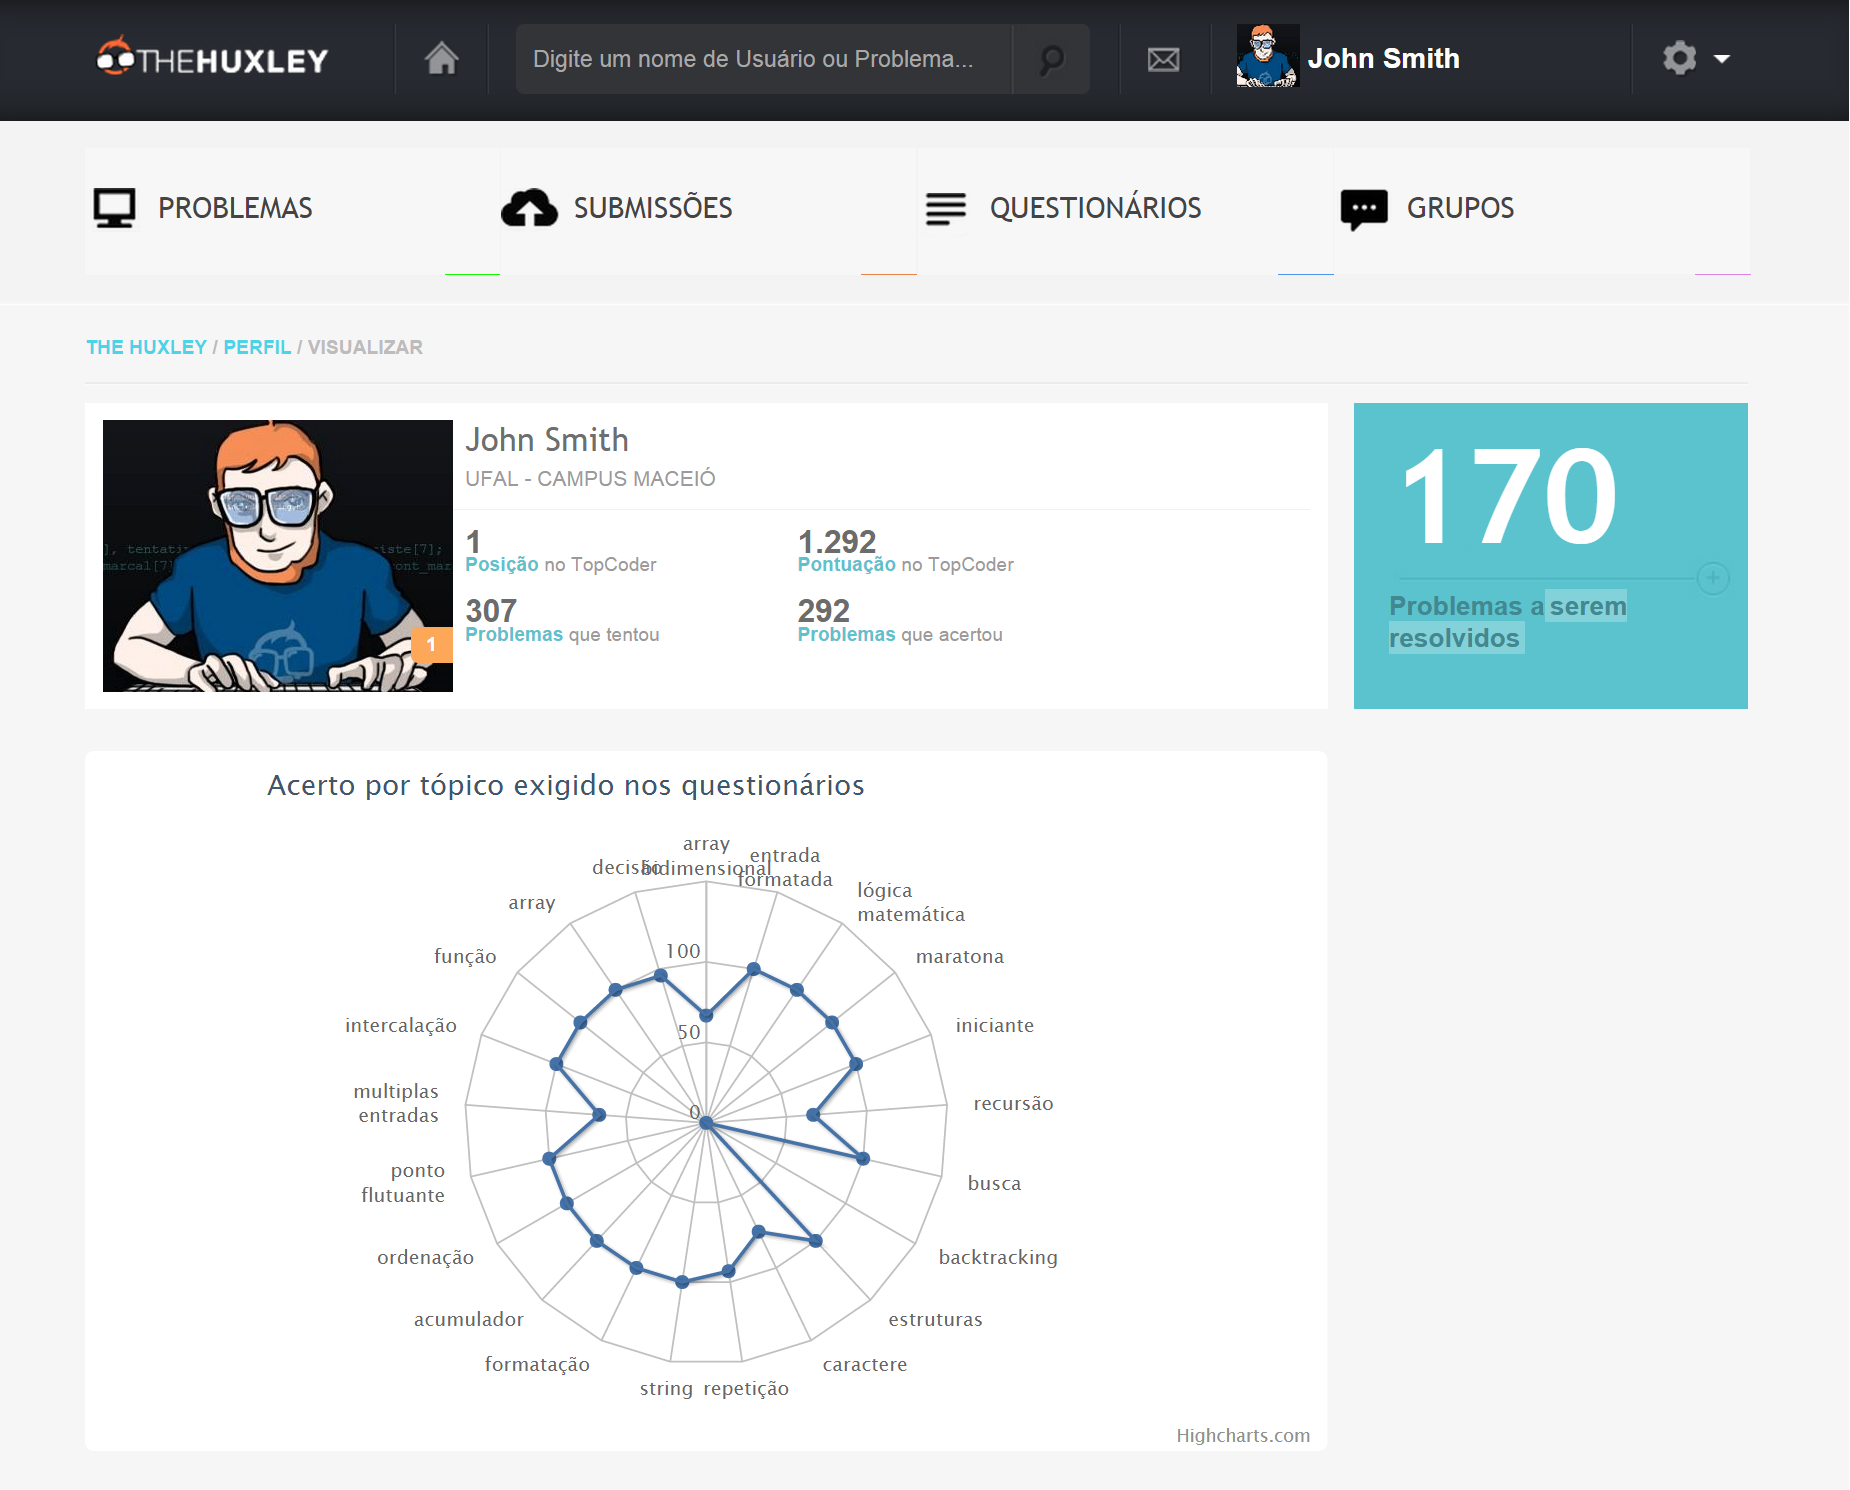
\includegraphics[width=.9\textwidth]{huxley.png}
\label{fig:huxley}
\end{figure}

Neste estudo, escolhemos utilizar o juiz online Huxley porque ele oferece funcionalidades suficientes para aplicação das métricas de identificação das soft skills do programador de software. Sua base de dados é a fonte para coleta dessas métricas. Além disso, temos acesso ao time de desenvolvimento e a alguns usuários do sistema, a saber, estudantes de programação da Universidade Federal de Alagoas.

Como exemplo de como podemos utilizar o Huxley para coletar métricas, podemos analisar os níveis de problemas que cada usuário resolve, o que nos oferece informações a respeito da habilidade Análise e resolução de problemas. Outro exemplo, como o sistema não penaliza submissões erradas, o usuário pode continuar tentando até conseguir, o que nos traz informações para verificar a habilidade Persistência.

\section{Métricas} 
\label{sec:metrics}

Como dito anteriormente, as métricas que propomos são alternativas que auxiliam na medição do nível de cada soft skill em um individuo de acordo com seu comportamento em atividades de programação. As soft skills que visamos medir são: Análise e resolução de problemas, Atenção a detalhes, Aprendizagem rápida, Persistência, Comunicação e Trabalho independente.

Cada métrica avalia uma soft skill com um valor no intervalo de zero a 100. Quanto maior o valor resultante da métrica para uma determinada soft skill, significa que o individuo possui essa habilidade mais desenvolvida. Dessa forma, se uma soft skill for medida em zero, significa que o indivíduo não possui essa habilidade. Se o valor for 100, ele possui a habilidade de uma maneira ótima. Escolhemos avaliar cada soft skill em um intervalo de zero a 100, para que fosse possível ordenar os resultados dos indivíduos e conhecer suas principais habilidades, bem como, as que precisam de melhoria.

A seguir, iremos apresentar as métricas para identificação de soft skills dos usuários do Huxley. Embora essas métricas tenham sido aplicadas a um sistema específico, elas também  podem ser empregadas em sistemas similares, ou seja, podem ser adaptadas para outros juízes online.

\subsection{Análise e resolução de problemas}

Para desenvolver as métricas de identificação automática dessas habilidades em um indivíduo, utilizamos sua interação com o sistema Huxley. Aqui propomos duas métricas, uma está relacionada com a habilidade de Resolução de problemas. A outra, está relacionada com Análise de problemas.

A métrica Resolução de problemas leva em conta a quantidade de soluções, ou seja, quantas submissões um usuário envia ao Huxley. Quanto mais um usuário envia submissões ao sistema, mais ele demonstra gostar de resolver problemas de programação. Por exemplo, dependendo do nível de dificuldade do problema, o usuário pode ter que apresentar diversas submissões ao sistema para conseguir resolvê-lo. No entanto, observe que isso não é necessariamente uma coisa ruim, por conta do processo de aprendizagem e prática de programação, que é a essência do Huxley. Enviar muitas submissões significa que o usuário está de alguma forma estudando e praticando programação continuamente.

Considere que $SUBMISSIONS$ é o número de submissões que o usuário enviou para o Huxley. 
Para fazer com que a métrica de Resolução de problemas seja avaliada de zero a 100, temos que tomar um valor de referência. Esse valor de referência é o número máximo de submissões que um usuário já enviou ao Huxley, chame de $SUBMISSIONS_{MAX}$. Assim, a métrica é calculada da seguinte forma:

\begin{equation} \label{m:resolucao}
\mbox{Resolução de problemas } = \frac{SUBMISSIONS}{SUBMISSIONS_{MAX}} * 100
\end{equation}

Portanto, o usuário que enviou mais soluções para o sistema vai pontuar 100 na habilidade de Resolução de problemas. A pontuação dos demais usuários será calculada relativamente a esse número máximo de submissões.

No entanto, quando consideramos apenas o número de submissões isoladamente, um elevado número de submissões erradas também pode significar que o aluno não está analisando muito bem o problema antes de tentar outras vezes. Dessa forma, propomos a métrica de Análise de problemas, considerando agora o número de submissões corretas, levando em consideração quantos problemas o usuário foi capaz de resolver e os níveis desses problemas.

Para cada submissão correta, o usuário do Huxley recebe uma pontuação dependendo do nível do problema que essa submissão responde. Por exemplo, quando um usuário resolve o problema de nível 1, ela ganha um ponto. Da mesma forma, se o problema é o nível 2, ele recebe 2 pontos. A pontuação máxima é 10, para submissões corretas de problemas nível 10.

Agora, dado que $CORRECT_{SCORE}$ é a soma das pontuações das submissões corretas do usuário. Além disso, dado que $SUBMISSIONS_{SCORE}$ é a soma das pontuações de todas as submissões do usuário. A métrica para Análise de problemas é:

\begin{equation} \label{m:analise}
\mbox{Análise de problemas } = \frac{CORRECT_{SCORE}}{SUBMISSIONS_{SCORE}} * 100
\end{equation}

Note que a métrica dessa soft skill pode ser avaliada entre zero e 100. Quanto mais o usuário envia submissões corretas, sua pontuação tende a 100. Caso contrário, se o usuário envia muitas submissões erradas, sua pontuação tende a zero.

\subsection{Atenção a detalhes}

Um indivíduo que presta atenção a detalhes é capaz de utilizar de forma completa todos os recursos disponíveis para realizar suas atividades. No contexto de um juiz online, o usuário atento precisa conhecer bem o sistema e saber como tirar proveito de todas as suas funcionalidades.

Por exemplo, para cada problema do Huxley existe um exemplo de entrada e saída na descrição do problema. Esta entrada e saída é o primeiro caso de teste que avalia cada submissão. Um usuário atento deve sempre observar cuidadosamente essa funcionalidade, para escrever sua submissão seguindo o exemplo. Com isso, ele evita apresentar soluções que falham no primeiro caso de teste.

Além disso, um usuário atento não apresenta submissões que causam erros de compilação, porque ele conhece os detalhes de sintaxe da linguagem que utiliza, e provavelmente testa seu código antes de submetê-lo.

Dessa forma, para identificar se um usuário possui a soft skill Atenção a detalhes, podemos analisar esses pontos. Para um usuário, seja $IO_{ERROR}$ o número de submissões que falham no primeiro caso de teste, e $SYNTAX_{ERROR}$ o número de submissões que foram avaliadas com erros de compilação. Seja ainda $SUBMISSIONS$ o número total de submissões por parte do usuário ao sistema. Definimos a métrica como se segue:

\begin{equation} \label{m:atencao}
\mbox{Atenção aos detalhes } = \left(1 - \frac {IO_{ERROR} + SYNTAX_{ERROR}}{SUBMISSIONS}\right) * 100
\end{equation}

Note que, se o usuário sempre envia submissões com erros de sintaxe ou erra no exemplo de entrada/saída, o quociente 
$\frac {IO_{ERROR} + SYNTAX_{ERROR}}{SUBMISSIONS}$ vale um. Portanto, a medida de Atenção a detalhes torna-se zero.
No entanto, se ele sempre está atento para evitar esses erros simples, o quociente passa a valer zero e a métrica de Atenção aos detalhes é avaliada em 100.

\subsection{Aprendizagem rápida}

Para identificar Aprendizagem rápida, é necessário estabelecer um critério de comparação, uma vez que essa soft skill diz respeito a capacidade de aprender em um tempo relativamente curto. No juiz online Huxley, os usuários estão agrupados por turma, equivalente a classe no curso de programação de que fazem parte. Para propor a métrica de aprendizagem rápida, estamos considerando a turma como fator comparativo.

No cálculo dessa métrica, primeiramente, determinamos para cada usuário do Huxley sua velocidade para resolver problemas, ou seja, para obter pontuação em submissões corretas. Tomamos a soma das pontuações das submissões corretas do usuário, $CORRECT_{score}$, para cada dia considerando dois dias diferentes e sequenciais ($DAY_0$ e $DAY_f$). Assim, a velocidade $SPEED$ para resolver problemas é dada por:

\begin{equation} \label{m:velocidade}
SPEED = \frac {CORRECT_{score} \mbox{ em } DAY_f - CORRECT_{score} \mbox{ em } DAY_0 }
              { \mbox{ Dias entre } DAY_0 \mbox{ e } DAY_f }
\end{equation}

% Continuamos cálculo da velocidade em uma janela de 6 meses. Depois disso, calcula-se a variação de velocidade para obter o ACC, o que vai significar a aceleração média de aprendizagem.

Precisamos ainda tomar um valor de referência para avaliar a métrica de Aprendizagem rápida entre zero e 100. Esse valor de referência é a velocidade máxima $SPEED_{MAX}$ obtida na turma. Em seguida, a métrica para esta soft skill é calculada da seguinte forma:

\begin{equation} \label{m:aprendizagem}
\mbox{Aprendizagem rápida } = \frac{SPEED}{SPEED_{MAX}} * 100
\end{equation}

Assim, o usuário que aprendeu mais rápido em cada grupo vai marcar 100. A pontuação dos demais é calculada relativamente a essa.

\subsection{Persistência}

Propomos a métrica de Persistência com base na quantidade de vezes que o usuário continua tentando resolver um problema. Quanto mais o usuário envia submissões, mais ele demonstra estar praticando continuamente. Mesmo que ele não esteja obtendo uma solução correta, está se esforçando e, eventualmente, irá conseguir acertar.
Esse comportamento está relacionado a persistência diante de adversidades na resolução do problema.

% Além disso, mesmo depois de uma solução correta, o usuário pode tentar submeter novamente, tentando melhorar o algoritmo. Esse tipo de comportamento também demonstra persistência.

Para medir a soft skill Persistência, considere que $CORRECT_{PROBLEMS}$ é número de problemas resolvidos por um usuário, excluindo os problemas que foram resolvidos corretamente na primeira tentativa. Considere ainda que $PROBLEMS$ é o número total de problemas que o usuário já tentou resolver, também sem contar os que foram acertados na primeira tentativa. Recomendamos não contar com esses problemas, porque como a solução foi obtida com apenas uma tentativa, o usuário não teve necessidade de demonstrar um comportamento persistente.

Aqui poderíamos dividir $CORRECT_{PROBLEMS}$ por $PROBLEMS$ para obter uma medida de Persistência.
No entanto, é interessante também levar em conta aqueles problemas que o usuário tentou várias vezes. Os quais, mesmo que ele que ainda não tenha obtido uma solução, pelo menos, tenha se esforçado para resolver. Então, calculamos a média de tentativas feitas pelos usuários até acertar cada problema do Huxley.

A partir disso, chame $EFFORT_{PROBLEMS}$ o número de problemas não resolvidos, mas que o número de tentativas foi acima da média de tentativas para cada um desses problemas. 
Por exemplo, se a média de tentativas até acertar o problema $\#1$ é $4$, e para o problema $\#2$ é $10$. Se o usuário tentou $5$ vezes, mais ainda não acertou o problema $\#1$, e o problema $\#2$, tentou $8$ vezes. O problema $\#1$ será contado em $EFFORT_{PROBLEMS}$. Mas o problema $\#2$ não será, pois o número de tentativas foi menor que a média de tentativas para resolver o problema.

Assim, propomos a métrica:

\begin{equation} \label{m:persistencia}
\mbox{Persistência } = \frac{ CORRECT_{PROBLEMS} + EFFORT_{PROBLEMS} }{ PROBLEMS } * 100
\end{equation}

Para alcançar a pontuação máxima em Persistência, que é 100, o usuário não deve deixar problemas sem solução correta, ou pelo menos ele tem que se esforçar, acima da média, para resolvê-los. Por outro lado, se um usuário deixa todos os problemas com soluções incorretas, sua pontuação em Persistência é zero.

\subsection{Comunicação}

No contexto de programação, propomos que alguém que tem habilidades de Comunicação escreve documentação de seus artefatos, costumando, por exemplo, comentar seus códigos-fonte. Além disso, no contexto de um sistema de juiz online, o indivíduo utiliza recursos de bate-papo para entrar em contato com outros usuários e participa em fóruns como objetivo ampliar sua comunidade.

Seria interessante fazer uso de todas essas características para definir a métrica de identificação da soft skill Comunicação. No entanto, o Huxley não possui as funcionalidade de bate-papo ou fórum. Por isso, optamos por apenas considerar os comentários de código-fonte.

Para um usuário, tomamos os arquivos de código-fonte de suas submissões corretas. Para cada arquivo selecionado, verificamos se ele possui comentários nas linhas de código. Seja $COMMENTED$ a quantidade de arquivos de código-fonte que tenham pelo menos um comentário, e $FILES$ o número de arquivos analisados. A métrica de Comunicação é definido como segue:

\begin{equation} \label{m:comunicacao}
\mbox{Comunicação } = \frac{ COMMENTED }{ FILES } * 100
\end{equation}

Note que, o valor da métrica está entre 0 e 100. Se o usuário costuma comentar seus arquivos de código-fonte, sua pontuação em Comunicação tende a 100. Por outro lado, se ele nunca comenta os códigos, sua pontuação em Comunicação é zero.

\subsection{Trabalho independente}

Sabemos que se alguém pode resolver problemas de programação com o mínimo de supervisão e não sente necessidade de pedir ajuda, mesmo diante de problemas de altos níveis de dificuldade, esse indivíduo sabe trabalhar de forma independente.

O Huxley oferece duas maneiras de pedir ajuda. Caso o usuário esteja com dúvidas diante de uma submissão, ele pode deixar uma pergunta no sistema, a qual será encaminhada ao professor responsável ou monitores de disciplina. O professor ou monitor, então, responde a dúvida escrevendo comentários para auxiliar na resolução do problema. Outra forma de pedir ajuda é quando um usuário tem uma submissão que não foi avaliada como correta. Nesse caso, o sistema oferece a oportunidade de ler uma dica, que é um comentário escrito pelo autor do problema informando qual foi o erro ou como obter a solução certa. No entanto, ler essa dica é opcional.

Seja $TIPS$ o número de submissões em que o usuário aceitou visualizar a dica e $HELPS$, o número de submissões em que o usuário pediu e recebeu comentários de ajuda. Chame $SUBMISSIONS$ o número de submissões do usuário. A métrica que representa Trabalho independente é dada por:

\begin{equation} \label{m:independente}
\mbox{Trabalho independente } = \left(1 - \frac {TIPS + HELP}{SUBMISSIONS}\right) * 100
\end{equation}

Observe que, se o usuário sempre visualiza dicas ou envia dúvidas e recebe ajuda para resolver os problemas, o quociente 
$\frac {TIPS + HELP}{SUBMISSIONS}$ vale um. Portanto, a medida de Trabalho independente torna-se zero.
O oposto disso é quando o usuário não necessita de ajuda ou dicas, de forma que o quociente passa a valer zero e a métrica de Trabalho independente é avaliada em 100.

\section{Aplicação de métricas utilizando a base de dados do juiz online}
\label{sec:exemplo-metricas}

Para ilustrar a aplicação das métricas propostas neste capítulo, observe a Tabela \ref{tab:dadosmetricas}. Nela mostramos os dados que coletamos para calcular as métricas de cada soft skill. Por motivos de privacidade, estamos apresentando dados de um usuário fictício, chamado John Smith.

\begin{table*}[h]
\footnotesize
\caption{\small Dados coletados para calcular as métricas} 
\addtolength{\tabcolsep}{-3.5pt}
\renewcommand{\arraystretch}{1.5} 
\centering

		\begin{tabular}{|p{9cm}|l|c|}\hline
		
        Informação & Variável & Dado \\\hline\hline
				
				\multicolumn{3}{|c|}{\textbf{Sobre o Huxley}} \\\hline
								
				Número máximo de submissões & $ SUBMISSIONS_{MAX}$	& 713 \\\hline\hline
				
				
				\multicolumn{3}{|c|}{\textbf{Sobre a turma de John Smith}} \\\hline
					
				Velocidade máxima de pontuação &  $ SPEED_{MAX}$ 	& 3,6 pontos/dia \\\hline\hline
				
				
				\multicolumn{3}{|c|}{\textbf{Sobre John Smith}} \\\hline
				
				Número de submissões 												& $ SUBMISSIONS$ 					& 647		\\\hline
				Soma das pontuações das submissões 					& $ SUBMISSIONS_{SCORE}$ 	& 2814	\\\hline
				%Número de submissões corretas 							& & 226		\\\hline
				Soma das pontuações das submissões corretas & $ CORRECT_{SCORE}$		 	& 681 	\\\hline
				
				
				Número de submissões com erro no exemplo de entrada e saída		& $ IO_{ERROR}$				& 86 		\\\hline
				Número de submissões com erro de sintaxe											& $ SYNTAX_{ERROR}$		& 9 		\\\hline
								
				Velocidade de pontuação																				& $ SPEED$						& 3,6 pontos/dia 	\\\hline
				
				Problemas tentados,
				sem contar os resolvidos na primeira tentativa				& $ PROBLEMS$ 								& 92		\\\hline
				Problemas resolvidos,
				sem contar os resolvidos na primeira tentativa				& $ CORRECT_{PROBLEMS}$ 			& 52		\\\hline
				Problemas não resolvidos,
				mas tentados por um número de vezes acima da média		& $ EFFORT_{PROBLEMS}$ 				& 10		\\\hline
				
				Número de códigos-fonte analisados										& $ FILES$ 										& 647		\\\hline
				Número de códigos-fonte comentados										& $ COMMENTED$ 								& 114		\\\hline
				
				Número de submissões com dica													& $ TIPS$ 										& 65		\\\hline
				Número de submissões com ajuda												& $ HELP$ 										& 4			\\\hline
				
					
     \end{tabular}
		\label{tab:dadosmetricas}
		%\fonte{}
\end{table*}

A partir dos dados coletados da base do Huxley, podemos então aplicar as métricas para identificar o nível de cada soft skill do usuário John Smith. Observe o exemplo dessa aplicação na Tabela \ref{tab:metricas}.

\begin{table*}[h]
\footnotesize
\caption{\small Métricas para identificar o nível das softs skills}
\addtolength{\tabcolsep}{-3.5pt}
\renewcommand{\arraystretch}{1.7} 
\centering

		\begin{tabular}{|p{4cm}|p{7cm}|p{3cm}|c|}\hline
		
        \textbf{Soft skill} & \textbf{Métrica} & \multicolumn{2}{c|}{\textbf{Valor}} \\\hline
													
				Resolução de problemas & $\frac{SUBMISSIONS}{SUBMISSIONS_{MAX}} * 100$
															 & $\frac{647}{713} * 100$ & 90,74 \\\hline
				
				Análise de problemas & $\frac{CORRECT_{SCORE}}{SUBMISSIONS_{SCORE}} * 100$
														 & $\frac{681}{2814} * 100$ & 24,20 \\\hline
				
				Atenção a detalhes & $\left(1 - \frac {IO_{ERROR} + SYNTAX_{ERROR}}{SUBMISSIONS}\right) * 100$
													 & $\left(1 - \frac {86 + 9}{647}\right) * 100$ & 85,32 \\\hline
				
				Aprendizagem rápida & $\frac{SPEED}{SPEED_{MAX}} * 100$
														& $\frac{3,6}{3,6} * 100$ & 100,00 \\\hline
				
				Persistência & $\frac{CORRECT_{PROBLEMS} + EFFORT_{PROBLEMS}}{PROBLEMS} * 100$
										 & $\frac{52 + 10}{92} * 100$ & 67,39 \\\hline
				
				Comunicação & $\frac{COMMENTED}{FILES} * 100$
										& $\frac{114}{647} * 100$ & 17,62	\\\hline
				
				Trabalho independente & $\left(1 - \frac {TIPS + HELP}{SUBMISSIONS}\right) * 100$
															& $\left(1 - \frac {65 + 4}{647}\right) * 100$ & 89,33 \\\hline
													
    \end{tabular}
		\label{tab:metricas}
		%\fonte{}
\end{table*}